\chapter[Estado da Arte]{Estado da Arte}

\section{Fases da Gamificação}
\label{sub:fasesgamification}
Todos os produtos que as pessoas utilizam na internet possuem diferentes
fases ao longo do seu ciclo de vida. Cada fase é reponsável por um tipo de contato diferente 
do usuário com a interface e com a imersão em que este está submetido.

Cada fase representa um sentimento diferente, uma experiência diferente
e uma nova forma de se lidar com aqueles atributos referentes ao que está
sendo lidado no procedimento de interação com o produto propriciado.

Essas fases que cada projeto é submetido já são conhecidos e desenhados. As fases
são quatro, bem claras e definidas. Elas são as seguintes:

\begin{enumerate}
    \item Descoberta;
    \item Reconhecimento;
    \item Construção;
    \item Fim de jogo.
\end{enumerate}

Essas fases circundam o ciclo de vida de um produto, desde o momento que este
é apresentado ao público até o momento que é deixado por ele. 

A definição das fases será ilustrada claramente nos subcapítulos que virão seguir.

\subsection{Descoberta}
\label{sub:descoperta}
É a fase onde o usuário não conhece sobre o produto, naõ tem noção de quais são os
seus objetivos nem como pode utilizá-lo. Esta é a fase onde o usuário tem o primeiro
contato, onde percebe como este funciona, bom como seus conceitos e valores.

Um exemplo de descoberta é uma apresentação de uma página no facebook, onde,
o novo produto será demostrado para grupos e nichos de interesse. A partir
de então, o usuário poderá passar a conhecer e utilizar o sistema.

Resumidamente, esta fase é reponsável por aprensentar o produto, fazer
com que os usuários o conheça.

\subsection{Reconhecimento}
\label{sub:reconhecimento}
Esta fase é reponsável por demonstrar ao usuário como o sistema se comporta.

Ela é essencial para que este entenda como o sistema funciona e o que cada
componente executa. Um exemplo bem conhecido desse procedimento é a utilização
de tutoriais e guias para novos usuários, no momento da sua chegada.

Ela termina quando o usuário está apto a continuar a utilizar o site sem
necessidade de aprender muitas outras novas ferramentas e funcionalidades.

Quando este está apto para tal, inicia-se a maior fase, onde o usuário
vai de fato entender e conhecer sobre o procedimento que está lidando.

\subsection{Construção}
\label{sub:constru_o}
Esta é a fase responsável pela real utilização do produto, onde as features
de fato serão utilizadas e irão agregar valor ao usuário.

Nesta parte o usuário já sabe e entende o papel de cada funcionalidade. Ele é capaz
de atingir os objetivos propostos. Aqui os recursos propostos serão utilizados
a depender na experiência e conexão do usuário com o produto.

Aqui tem que ser criados gatilhos para que mantenha o usuário constantemente utilizando
o sitema de acordo com o planejado.

\subsection{Fim de Jogo}
\label{sub:fim_de_jogo}
Toda aplicação desenvolvida passa pela fase de partida, onde está é totalmente utilizada
e de alguma forma, o usuário a deixará. 

Não necessariamente deixará de utilizar e participar do envovilmento total proposto pela
organização. Um exemplo disto é um jogo desenvolvido. Quando o primeiro jogo acabar, o
usuário passará pela fase de fim de jogo, que pode deixar o usuário motivado a se conectar
e adquirir a próxima versão do jogo que será lançada futuramente.

É importante que seja feito corretamente o desfeixo do produto para que uma linhagem seja
prosseguida.


Todas essas diretivas e fases que existem dentro do ciclo de vida de um produto deve ser
tratadas de forma independente e diferente entre si. Agora pode-se indagar onde a gamificação
entre neste processo, sendo que cada fase deve ser tratada de uma forma diferente pelo
usuário e, consecutivamente, por parte de quem está a oferecer o produto.

Assim, há a necessidade de que a gamificação também seja moldada conforme o objetivo de
cada fase a ser aplicada.

Dessa forma, cada fase implementada será pensada e avaliada para que seja possível a
aplicação de um  projeto de gamificação. Cada fase terá um foco em motivações
básicas diferentes, que propiciarão uma experiência diferente para o usuário.

A figura \ref{fig:fasesoctalysis} ilustra um exemplo do como pode ser aplicado na
Rede Social About a gamificação ao longo das quatro fases.

\begin{figure}[h]
    \centering
    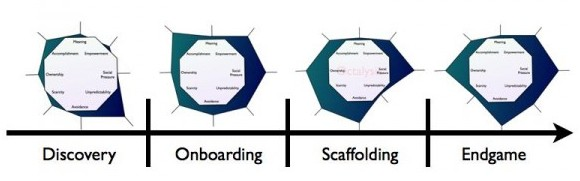
\includegraphics[width=400px, scale=1]{figuras/fasesoctalysis}
    \caption{Fases do Octalysis}
    \label{fig:fasesoctalysis}
\end{figure}

Como pode ser visto na figura \ref{fig:fasesoctalysis}, são projetados vários
desenhos e desings modificados e diferentes para cada fase. Cada uma destas
tem um pensamento e objetivo diferente.

Na fase de descoberta, pode ser visto que a motivação básica mais presente é
a imprevisão e a curiosidade. O que dá margem para que o usuário imagine diferentes
possibilidades sobre o produto. 

No momento de uma propaganda, por exemplo, este lado do framework pode gerar uma
extrema curiosidade no usuário, o que fará com que ele fique motivado a procurar
e entender mais sobre o que está sendo anunciado.

Isto pode ser extremamente importante para conseguir capturar novos usuários.

Na segunda fase, em que o usuário vai conhecer sobre o produto, pode ser visto
que as fases relativas a desenvolvimento próprio e realização de si mesmo
são bem mais presentes.

Este ponto pode ser aplicado, pois o usuário irá se sentir realizado e inteligente
ao oberservar seu desenvolvimento próprio elevado. Isto irá gerar um prazer em fazê-lo
sentir o quanto pode ser bom em realizar as tarefas que a ele estão sendo designadas
no início do procedimento.

Na terceira fase é possível verificar que duas motivações básicas são muito presentes:

\begin{itemize}
    \item Motivação Básica Cinco: Influência e Dinâmica Social;
    \item Motivação Básica Seis: Escassez e Impaciência.
\end{itemize}


Para a Motivação Básica Cinco, isto deixa o usuário motivado ao utilizar o produto
por sentir que está exercendo uma alta influência social, que está envolvido em
uma dinâmica social que faz influência em outras pessoas.

Isto faz com que o usuário fique motivado a continuar engajado no processo, pois,
este estará conseguindo perceber o quanto está sendo participativo no meio social
e que o produto está sendo proveitoso por fazê-lo se sentir socialmente influente
e participativo.


A segunda motivação básica vizualizada nesta fase, Escassez e Impaciência, acontece
pois é possível verificar que o usuário fique motivado a executar determinadas
tarefas baseado neste sentimento.

Esta o deixará preocupado com a questão de não cumprir corretamente os objetivos.
Esta fase é responsável por fazê-lo se sentir em um meio escasso caso não execute
os objetivos propostos.

Isto vai motivar o usuário e vai fazer com que faça o necessário para que não
sinta estes sentimentos.

A última fase, fim de jogo, também tem sua motivação básica predominante que
a guia. Esta é guiada pela Motivação Básica Oito: Perca e evitação.

Esta irá gerar um sentimento que faz o usuário se sentir mal. Este sentimento
envolve o fato de que o usuário pode perder o todo o processo que foi executado.


Este é um sentimento ruim. Sentimento qual o usuário não deseja sentir. Para tanto
ele se esforçará a fim de não presenciar as experiências que são submetidas.

Como pode ser visto, estes procedimentos de cada fase são extremamente aplicáveis
e úteis para que o usuário tenha várias experiências ao longo do clico de vida do
produto. O que propiciará uma experiência muito mais agradável.

Dessa forma, serão desenhados quatro frameworks diferentes para a Rede Social About.
Uma para cada fase diferente do produto, onde serão estudadas separadamente para
aplicá-las e possibilitar uma boa experiência para o usuário.

\section{Octalysis Strategy Dashboard}
\label{sec:octalysisdashborad}
O framework octalysis oferece suporte para a construção de um projeto de gamificação
bem estruturado e baseado em necessidades do domínio do problema.

Este suporte se trata do Octalysis Strategy Dashboard, o qual pode ser analisado as
estretégias de mergado, perspectiva do usuário, intenções desejadas para a gamificação,
mecanismos de feedback e incentivos.

Existem processos sistematizados para estabelecer cada fase e como será dado o 
resultado da gamificação. 

Para este trabalho, serão utilizados estes procedimentos sistematizados. 

Para ilustrar a metodologia de estratégia do octalysis dashboard, será representada
a figura a seguir, que contém a metodologia e a formalização da sua construção.

A seguir serão descritos sub capítulos, que retratarão o papel e a utilidade de cada
componente.


 \begin{figure}[h]
     \centering

     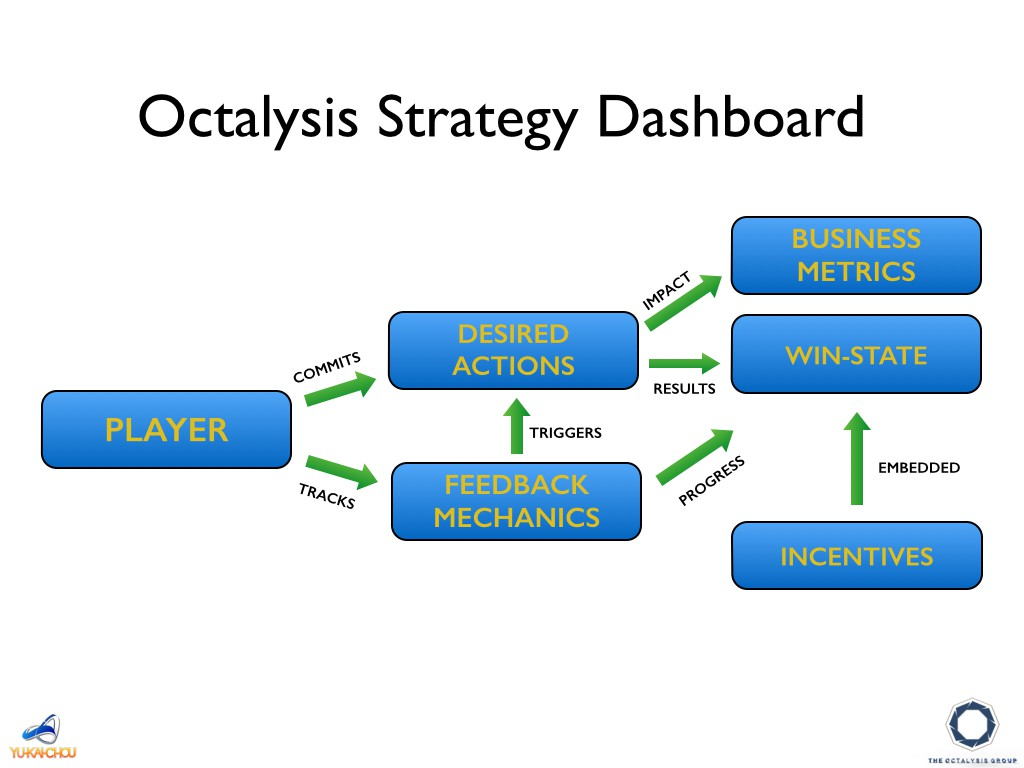
\includegraphics[width=450px, scale=1]{figuras/dashboard}
     \caption{Octalysis Strategy Dashboard}

     \label{fig:dashboard}
 \end{figure}

\subsection{Business Metrics}
\label{sub:business_metrics}
As métricas de negócio, em português, são termos quantitativos que podem ser utilizados
para ter um número palpaável sobre como está um determinado ponto do projeto de gamificação
que teve como o objetivo de ser atacado.

Essas métricas, irão auxiliar a verificarmos o quanto a aplicação da gamificação foi eficaz ou
não dentro de um determinado objetivo.

Alguns exêmplos de técnica de gamificação que serão utilizadas estão a seguir:

\begin{itemize}
    \item Aumentar o número de seguidores dos usuários prêmio
    \item Aumentar o número de vendas de um livro sobre o produto
    \item Aumentar o número de inscritos na rede social
    \item Aumentar a quantidade de acessos diários
    \item Aumentar os seguidores escritos
    \item Aumentar os usuários que compartilham conteúdos pelas redes sociais
    \item Aumentar a quantidade de curtidas em determinado post
\end{itemize}

Estes exemplos de métricas serão submetidos à Rede Social About antes da apresentação da
gamificação. E assim que determinada técnica for utilizada, será então executada uma
segunda medição, que propiciará analisar as diferenças entre os resultados obtidos.

\subsection{Define User Types}
\label{sub:define_user_types}
Este ponto do dashboard, para definir os tipos dos usuários, é responsável por conseguir
elaborar e definir quais são os tipos de usuários que serão aumejados e trabalhados, quando
falamos sobre gamificação.

Esta fase é um processo de definição de nicho sobre onde a gamificação vai atuar, quanto a
usuários, dentro da Rede Social About? Quais serão os passos utilizados para que este público
seja atingindo?

Alguns exemplos de tipos de usuário se encontram a seguir:

\begin{itemize}
    \item Companhias que desejam que seus trabalhadores atinjam determinadas métricas
        ao fim de cada mês;
    \item Educadores e políticos que querem utilizar conhecimento para criar impáctos
        sociais;
    \item Indivíduos que são apaixonados por gamificação, games e desenvolvimento próprio.
\end{itemize}
 
Desta maneira, será possível realizar um projeto de gamificação focado ao definir o tipo
de usuários. Pois, a partir daí, será possível identificar quais caminhos são mais vantajasos
quanto a escolha das motivações básicas que serão utilizadas ao longo das quatro fases.

\subsection{Define Desired Actions}
\label{sub:define_desired_actions}
A definição das ações desejadas são todas as iniciativas tomadas pelo usuário que o levam a caminhar para
o Win Stade(Estado de Vitória), seja ela em qual fase for. Sendo assim, a Rede Social
About terá alguns pontos que serão definidos como os desejados. Estes serão desenhados
até que o estado de vitória seja definido. Assim, para as quatro fases serão definidas
ações diferentes. Alguns exemplos de ações que podem ser escolhidas serão apresentadas
a seguir.

Ações na fase da descoberta:
\begin{itemize}
    \item Conhecer a Rede Social About;
    \item Clicar no link da Rede Social About
    \item Conhecer as features oferecidas pela Rede Social
\end{itemize}


Ações na fase de reconhecimento do projeto: 
\begin{itemize}
    \item Executar o tutorial de uso da About;
    \item Compartilhar a Rede Social About com os amigos
    \item Adicionar foto e email na network
    \item Permitir a escrição na lista de email
\end{itemize}

Já para a fase de construção do projeto, os seguintes pontos podem ser um
exêmplo:

\begin{itemize}
    \item Fazer login diariamente na network
    \item Abrir semanalmente os emails enviados pela network
    \item Compartilhar abouts com os amigos
    \item Participar de grupos no facebook sobre a rede social about
    \item Adquirir a versão prêmio da rede social about
    \item Inscrever em grupos de discussão sobre a rede social about
    \item Escrever mais de um about diariamente
    \item Votar em mais de vinte abouts diarios
\end{itemize}

Por fim, na fase de fim de jogo, alguns exemplos de construção podem ser dados. Eles são os seguintes:
\begin{itemize}
    \item Se tornar contribuidor da Rede Social About;
    \item Fazer parte da equipe de desenvolvedores da About
    \item Propor melhorias para a about
    \item Tornar-se moderador dos abouts
\end{itemize}

Estes exemplos ajudam e exclarecer como os objetivos podem ser alcançados. Elas definem um nível de
granularidade maior.

\subsection{Define Feedback Mechanics}
\label{sub:define_feedback_mechanics}
A definição de mecanismos de feedback são extremamente importantes para a exeperiência do usuário
com a network. Este é responsável por ilustrar e deixar bem claro para o usuário, como ele está
prosseguindo no desenvolvimento do projeto.

Atualmente os usuários tem requirido feedbacks constantes, em tempo real, para as suas ações
realizadas. Sendo assim, é necessário que existam esses gatilhos em vários pontos da
Rede Social About e que o usuário possa entender rapidamente.

A seguir estão alguns exêmplos de como podem ser exclarecidos esses feedbacks para o usuário:

\begin{itemize}
    \item Countdown Timers
    \item Desbloquear conteúdo da página
    \item Status de progresso na sidebar
    \item Verificação de qual era a melhor escolha
    \item Vídeo embutido
    \item Barra de pontos de status
    \item Certificados
    \item Medalhas
    \item Gráficos de desempenho
\end{itemize}

Assim, com exemplos dessa maneira, é possível que o usuário verifique o quanto suas atividades estão
sendo aproveitadas.

\section{Incentives And Rewards}
\label{sub:incentives_and_rewards}
O sistema de incentivos e recompensas fecham o ciclo do dash board, que fazem com que 
os usuários se sitam motivados a alcançar cada estado de vitória. Eles ajudam a indicar
o quanto ainda falta para que o estado seja aumejado.

\begin{itemize}
    \item Status Points
    \item Símbolos de vitórias
    \item Conhecer os desenvolvedores da about
    \item Ter acesso a arquivos confidenciais
    \item Descontos nos produtos
\end{itemize}

\section{Objetos de Gamificação}
\label{sec:objetodegamificacao}
Os objetos de gamificação serão os pontos da rede social em será aplicado o framework,
com os objetivos de atingir alguma meta de negócio.

Os objetivos de gamificação são os seguintes:

\begin{itemize}
    \item Fazer com que o usuário escreva mais abouts;
    \item Fazer com que o usuário julgue mais abouts;
    \item Fazer com que o usuário convide amigos que não estão cadastrados na about;
\end{itemize}
